%!TeX root = Chapter_IceTheory2
\documentclass[../../CompleteThesis2/Complete_2ndDraft]{subfiles}
%\graphicspath{{../../Figures/}}
\begin{document}



\section[Water Isotopes][Water Isotopes]{Water Isotopes}
\label{Sec:Ice_WaterIsotopes}

A corner stone in ice core analysis, which helps lay the basis for paleo climate research, is the measurements of isotopic composition of the water which makes up the ice or of the encapsulated air in bubbles throughout the ice. Water isotopes are sensitive to temperature changes and can thus be used as a proxy for paleo temperature and climate along with being used as dating parameters, since the annual cycles often are detectable in water isotope data, as is clearly the case with the water isotopic ratios depicted in Figure \ref{Fig:ICE_Crete_10m_dated}.

\begin{figure}[h]
	\centering
	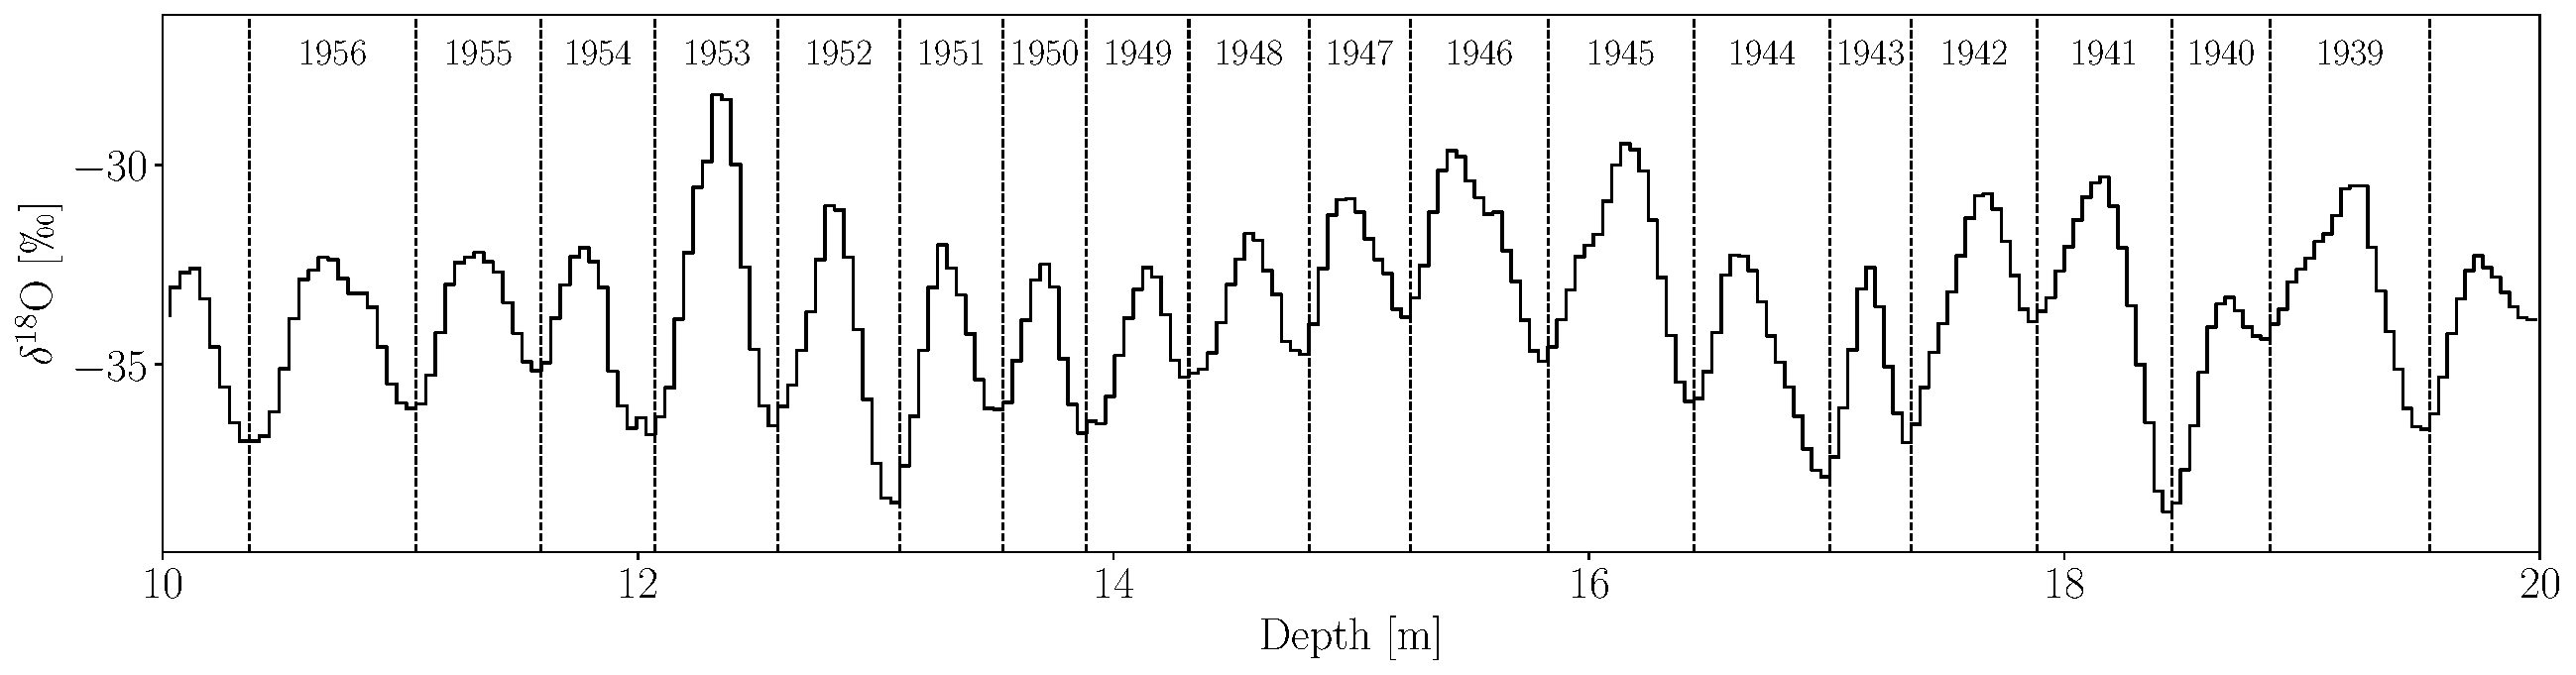
\includegraphics[width=\textwidth]{Crete_10m_dated.pdf}
	\caption[10 m of Crête ice core with dating.]{\small Ten meters of the top of Cretê ice core, with identification and dating of 19 annual layers.}
	\label{Fig:ICE_Crete_10m_dated}
\end{figure}


\subsection[$\delta$ Notation]{$\delta$ Notation}
\label{Subsec:Ice_WaterIsotopes_deltaNotation}
\begin{marginfigure}
	\centering
	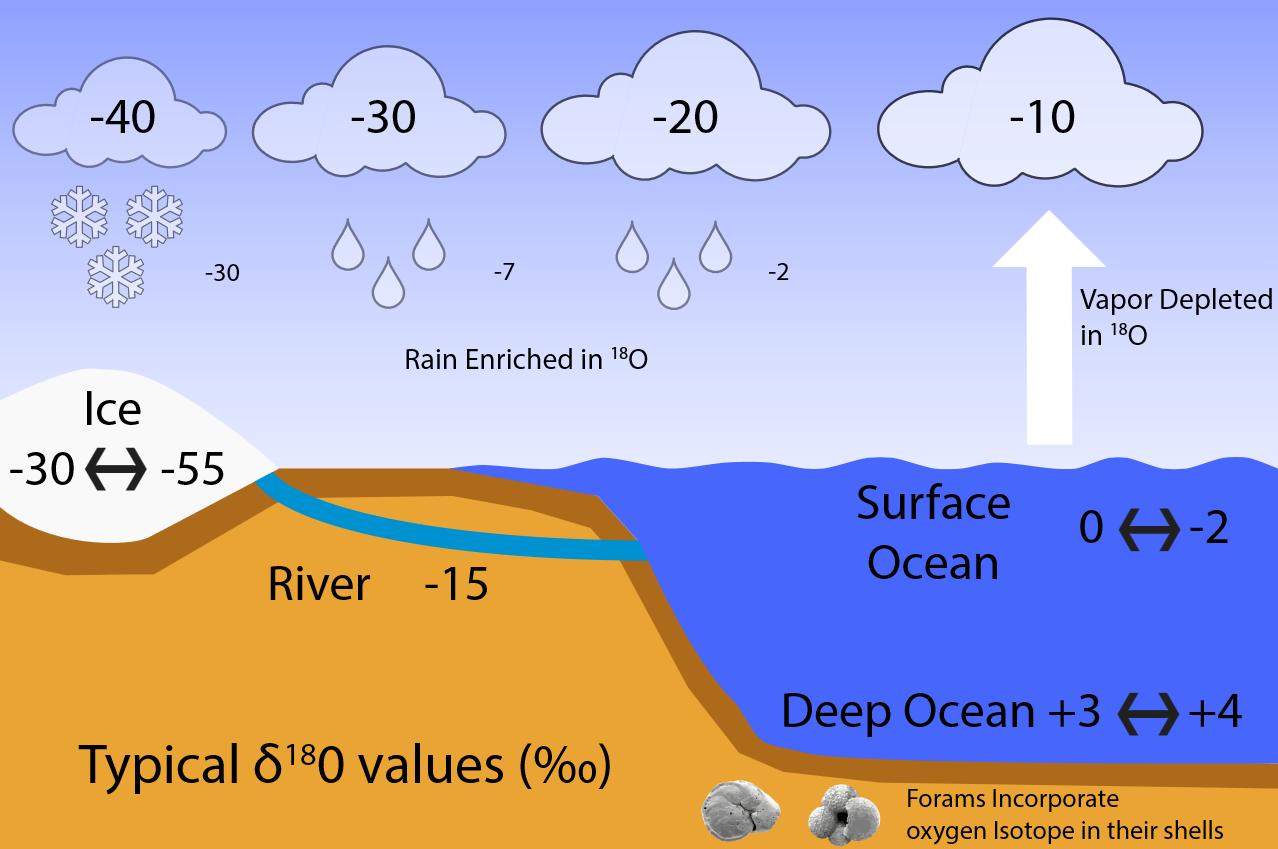
\includegraphics[width=\marginparwidth]{Fractionation.png}
	\caption[Fractionation]{\footnotesize Fractionation through evaporation, transportation and precipitation along with typical water isotopic ratios.}
	\label{Fig:ICE_ISO_Fractionation}
\end{marginfigure}
Water isotopic ratios, i.e. the ratio of the minority isotope, ${\text{H}_2^{18}\text{O}}$ or ${\text{H}_2^{17}\text{O}}$ ($^2\text{H}_2\text{O}$), compared to the majority isotope, ${\text{H}_2^{16}\text{O}}$ ($^1\text{H}_2\text{O}$), are used to report the quantities of isotopes in a sample relative to the ratio of a given reference water sample. This is commonly expressed in the $\delta$-notation as:
\begin{equation}
	\delta^i = \frac{^iR_{sample}}{^iR_{reference}} - 1		
\end{equation}
where $^{18}R = \frac{n_{^{18}\text{O}}}{n_{^{16}\text{O}}}$, $^{2}R = \frac{n_{^{2}\text{H}}}{n_{^{1}\text{H}}}$  and $^{17}R = \frac{n_{^{17}\text{O}}}{n_{^{16}\text{O}}}$. Here $n$ is the abundance of the given isotope.%\todo{ICE-ISO: Implement illustration of fractionation and deposition}

Besides the isotopic quantities $\delta^{17}\text{O}$, $\delta^{18}\text{O}$ and $\delta^2\text{H} = \delta\text{D}$, both deuterium excess and $\Delta^{17}\text{O}$, known as $^{17}\text{O}$ excess, can be of interest. Deuterium excess is often used as a measure of the kinetic fractionation processes, taking place in the water vapor formation of polar precipitation, to which it is especially sensitive, giving an indicator of the conditions during precipitation formation, and thus giving a pointer to the source of the water vapor.

Like deuterium excess $^{17}\text{O}$ is sensitive to kinetic fractionation, but much less sensitive to equilibrium fractionation than both $\delta$D and $\delta^{18}$O. Along with being nearly insensitive to temperature(REFERENCES), these robustness factors leads to $^{17}$O being usable as an independent parameter to be used to reveal the ways of the complicated mixing effects of fractionation due to evaporation, transportation, formation and deposition.

The naturally occurring oxygen isotopes are approximately divided into 99.759\% $^{16}\text{O}$, 0.037\% $^{17}\text{O}$ and 0.204 \% $^{18}\text{O}$, and historically the focus has been on the water isotopic ratio of $\delta^{18}$O, due to the higher abundance making it easier to measure than for example $\delta^{17}$O. One of the challenges of modern glaciology is to develop a stable, precise and accurate measuring technique for $\delta^{17}$O. This work examines the data from ice cores drilled and measured in the past century, and only $\delta^{18}$O has been measured for these cores.

\subsection[Relation to Temperature]{Water Isotopes in the Earth System}
\label{Subsec:Ice_WaterIsotopes_EarthSystem}


Due to H$_2^{18}$O being slightly heavier than H$_2^{16}$O, the isotopic signal is depleted of the heavier isotopes through transportation of the water vapor before it is deposited at the ice sheets. A clear annual signal in the $\delta^{18}$O measurements can be observed due to the seasonal temperature changes from summer to winter at deposition time. This is the main isotopic feature under consideration for this thesis. The greatest issue with this type of signal is that there is a loss of information over time as the snow becomes more compact and diffusion processes wash out some of the signal throughout the ice depth. Thus to be able to examine and analyze isotopic signals more accurate and precisely, the processes of densification and diffusion need to be well understood.

%\begin{itemize}
%	\item Temperature and accumulation
%	\item Transportation and deposition
%	\item Thermodynamics(?)
%\end{itemize}


\section[Densification and Diffusion][Densification and Diffusion]{Densification and Diffusion}
\label{Sec:Ice_DensificationAndDiffusion}
Deposited snow will over time be compressed and at last be compacted completely to glacial ice, see Figure \ref{Fig:ICE_DENS_FirnColumn}. Any ice state between snow and glacial ice is referred to as \textit{firn}. Throughout the firn column the important processes of densification and diffusion take place. Both processes need to be well understood and examined when analyzing ice core data, as diffusion and densification play a large role in thinning of annual layers due to compression of snow to ice and in washing out the measured signals through diffusion in the firn. Specifically in this thesis the diffusion processes are carefully examined, as the diffusion length, $\sigma$ can be used as a proxy for paleotemperatures.

\begin{marginfigure}
	\centering
	\includegraphics[width=\marginparwidth]{firn_popular.jpg}
	\caption[Densification process]{\footnotesize Illustration of the densification process of a firn column, from snow deposition to glacial ice.}
	\label{Fig:ICE_DENS_FirnColumn}
\end{marginfigure}

\subsection[Densification][Densification]{Densification}
\label{Subsec:Ice_DiffusionAndDensification_Densification}
Densification is the process of compression of snow to ice. It affects the annual layer thickness in the data as snow will be compacted to a smaller volume under pressure from the firn column above until it reaches a solid ice state with an, almost, constant density.

Commonly three stages of densification are described in the firn column. The first stage is between the initial precipitated snow density and the 'critical density' at $0.55 \frac{\text{Mg}}{\text{m}^3}$, the second stage is between critical density and the close-off density at $0.82-0.84 \frac{\text{Mg}}{\text{m}^3}$, and the third stage is from close-off and all the way through the glacial ice. The close-off depth refers to the depth, where all air pores in the firn column become closed-off from the atmosphere at the surface, and separate bubbles start to form in the ice.

At the first stage the densification is mostly due to grain settling and packing and the densification rate is very rapid. At the second stage, the snow is close to isolating air bubbles. At the third stage, the dominating densification taking place is by the compression of air bubbles.\\
For these three stages it has early been of interest to develop a model to determine the depth-density profile, which is dependent on snow accumulation rate and temperature. The focus was on developing an empirical model for the first and second stages of densification, as they are the most dramatic sections of the firn column considering densification and diffusion.

A number of different densification models have been developed (REFERENCES),  but for this thesis work, only one model is used, namely the Herron-Langway empirical model, first presented by Michael M. Herron and Chester C. Langway Jr in \cite[Herron and Langway, 1980]{HerronLangway1980}. The basic idea of the model will be presented in the following. For a more thorough mathematical presentation, the reader is referred to Appendix \ref{AppIIX:HLmodel} or the original paper.

\subsubsection[HL in This Thesis]{Herron-Langway Model in This Thesis}
\label{Subsubsec:Ice_DiffusionAndDensification_Densification_HLmodel}
The Herron-Langway model(from now on \textit{HL model}), is an attempt to describe the densification process through a firn column, given some initial conditions, mainly the temperature and annual accumulation rate at the site. The model is generally derived from the suggestion that during the process of densification, the proportional change in airspace is linearly related to the change in stress due to the overburdened snow:
\begin{equation}
	\frac{\text{d}\rho}{\rho_{\text{ice}} - \rho} = \text{const.} \rho \, dh.
	\label{Eq:HL}
\end{equation}
with $\rho$ being the density of the firn, $\rho_{\text{ice}}$ the density of glacial ice and $h$ the depth.

This implies, by integration, a linear relationship between $\left[\frac{\rho}{\rho_{\text{ice}} - \rho}\right]$ and $h$. Through empirical analysis of depth-density measurements from a number of different ice cores, and the basic acceptance of Equation \ref{Eq:HL}, the rate equations $\left(\frac{\text{d}\rho}{\text{d}t}\right)_{\text{zone 1}}$ and $\left(\frac{\text{d}\rho}{\text{d}t}\right)_{\text{zone 2}}$ can be derived, see Appendix \ref{AppIIX:HLmodel}. From these rate equations, and given temperature, $T$, accumulation rate, $A$, and initial snow density, $\rho_0$, it is then possible to estimate the density and age of the snow at any given depth. 

In this thesis, the HL model is used to generate an estimate of the density profile for each ice core site under examination. The HL model has been incorporated in the computational works of this thesis as a class module, which computes a diffusion length profile, given initial parameters. An example of five different density profiles computed with this module, given present day conditions at five different ice core drilling sites as initial conditions can be seen in Figure \ref{Fig:DensProf_Examples}. These profiles are then used to give a first diffusion length profile estimate for each core, which is used in the further analysis. 
\begin{marginfigure}
	\centering
	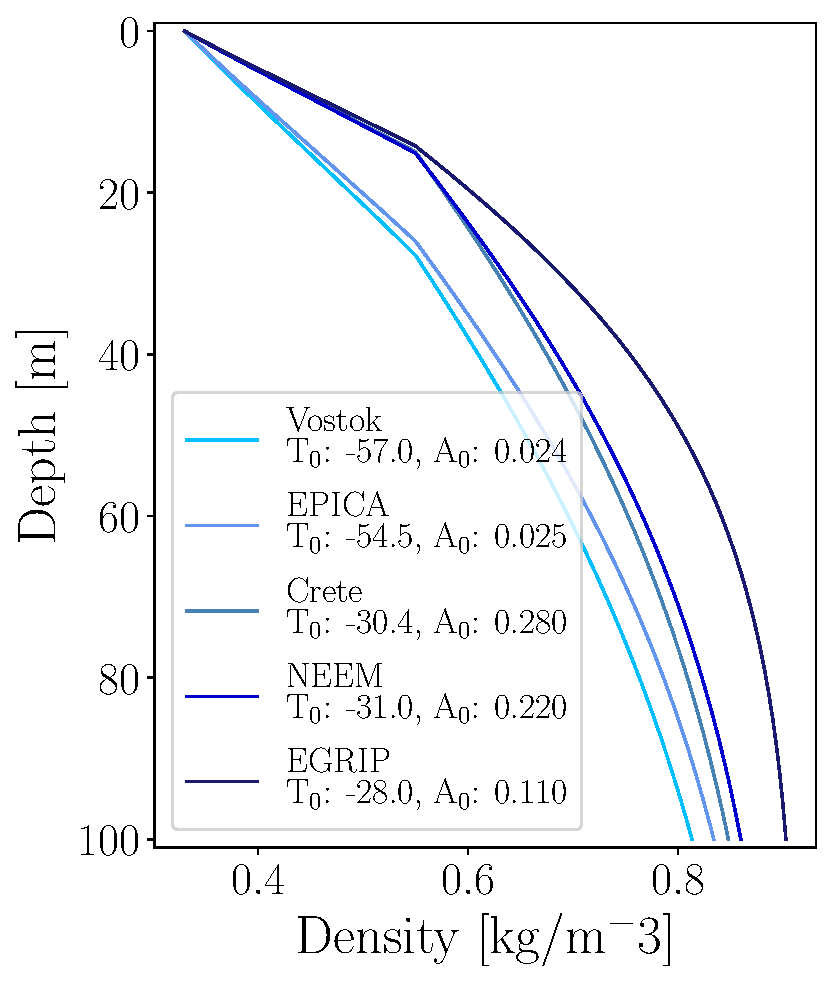
\includegraphics[width=\marginparwidth]{DensProf_Examples.pdf}
	\caption[Five theoretical density profile examples.]{\footnotesize Density profile examples given five different initial conditions representing present day conditions at the five different ice core locations. Temperature, $T_0$, is in $^{\text{o}}$C and accumulation, $A_0$, is in meter of water equivalent per year.}
	\label{Fig:DensProf_Examples}
\end{marginfigure}
For the purpose of this thesis, an extra module has been added to the HL model class, which makes it possible to incorporate any measured data in the density profile estimation, so as to best approach the actual profile at the drilling site. This module is implemented by allowing an intake of two arrays consisting of depth and density measurements, which are then used to fit the model, using a least square optimization from \lstinline[language=python]|scipy|, \lstinline[language=python]|scipy.optimize.leastsq|. An example of a density profile estimation, both using the measured data and using only the model, can be seen in Figure \ref{Fig:DensProf_Examples_SiteA_wData}.
\begin{marginfigure}
	\centering
	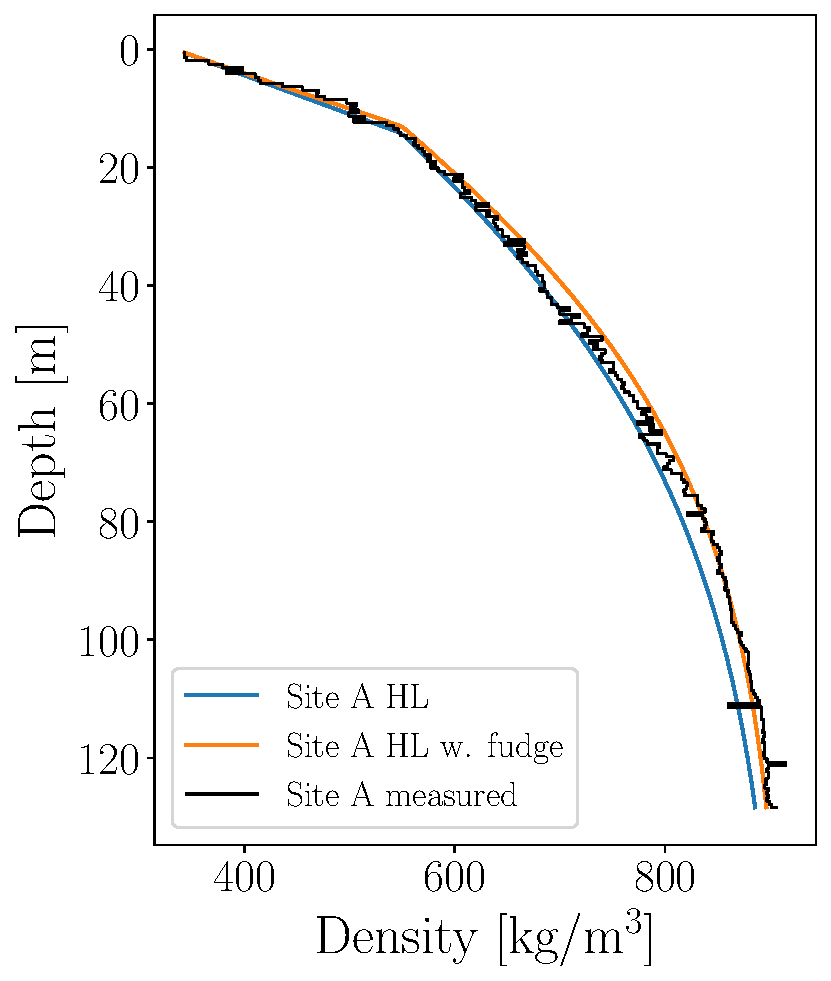
\includegraphics[width=\marginparwidth]{SiteA_DensProfile_wHL.pdf}
	\caption[Site A density profile, data and theory.]{\footnotesize Density profiles from ice core Site A near Crête. Both purely modelled profile and profile fitted to the inputted depth-density measurements are presented.}
	\label{Fig:DensProf_Examples_SiteA_wData}
\end{marginfigure}




\subsection[Diffusion]{Diffusion}
\label{Subsec:Ice_DiffusionAndDensification_Diffusion}
In general diffusion refers to the mixing of material, e.g. molecules, by net movement from high to low concentration due to somewhat random stochastic processes. When considering ice cores, the diffusion taking place is the displacement of the molecules that make up the ice and firn, for example water molecules. The diffusion processes are subject to varying conditions and are caused by different effects at different depths. In the first few meters of an ice core, the main diffusion is due to mixing and settling of snow particles due to surface conditions and gravity, and later, the total diffusion is more subject isotopic gradients in the ice. 

The diffusion processes are different for the porous firn and for the later glacial ice, described in the different stages above and below close-off depth.

\subsubsection{In Firn}
\label{Subsubsec:Ice_DiffusionAndDensification_Diffusion_Firn}
The diffusion processes in firn can be used to describe the attenuation of a given signal, e.g. a water isotopic signal, due to vapor phase diffusion in the porous firn column. This vapor phase process takes place in the air pockets of the material from time of deposition to pore close-off. 

To develop accurate knowledge of paleo climate and temperatures it is of great importance to understand this process, as a reconstruction of the part of the signal lost will reveal finer details in the signal and thus a more detailed knowledge of past times. 

Diffusion is modeled through Fick's $2^{\text{nd}}$ law, which describes the change in concentration of a substance with time, due to diffusion:
\begin{equation}
	\frac{\partial \phi}{\partial t} = D(t) \frac{\partial^2 \phi}{\partial z^2} - \dot{\epsilon}_z(t) z \frac{\partial \phi}{\partial z}
	\label{Eq:Fick2_concentration}
\end{equation}

Focusing on water isotopic ratios, the water isotopic signal can be assumed as a concentration, $\phi \rightarrow \delta$, resulting in a diffusion equation as:
\begin{equation}
	\frac{\partial \delta}{\partial t} = D(t) \frac{\partial^2 \delta}{\partial z^2} - \dot{\epsilon}_z(t) z \frac{\partial \delta}{\partial z}
	\label{Eq:Fick2_WIS}
\end{equation}

Through depth and time driven attenuation due to diffusion there is a loss of information which can be used to gain information of the underlying processes. Since the diffusion constant and the vertical strain rate $\dot{\epsilon}_z(t)$ in Fick's $2^{\text{nd}}$ law are dependent on temperature and accumulation on site, the information loss process can infer the temperature of firn and accumulation on site.

The attenuated, directly measured, isotopic signal, $\delta(z)$, can be described as the convolution between the initial isotopic signal, $\delta '(z)$, and a Gaussian filter, $\mathcal{G}(z)$. The Gaussian function describes the stochastic diffusion process. The signal is furthermore multiplied by the thinning function, $S(z)$, which describes the total thinning of a given layer at depth $z$ due to the vertical strain from the above firn column.:
\begin{equation}
	\delta(z) = S(z)[\delta'(z)*\mathcal{G}(z)]
	\label{Eq:diff_solution_conv}
\end{equation}
where
\begin{equation}
	S(z) = e^{\int_{0}^{z}\dot{\epsilon}_z(z')\, dz'}
	\label{Eq:Thinning_fct}
\end{equation}
and
\begin{equation}
	\mathcal{G}(z) = \frac{1}{\sigma\sqrt{2\pi}}e^{-\frac{z^2}{2\sigma^2}}
	\label{Eq:Gauss_filter}
\end{equation}

In the Gaussian filter, the variance $\sigma^2$ is referred to commonly as the diffusion length: the distance a water molecule is displaced along the z-axis. This quantity is directly related to both $D(t)$ and $\dot{\epsilon}_z(t)$(the strain rate being approximately proportional to the densification rate in the column). Thus an accurate estimate of the diffusion length is crucial for describing the diffusion process.
The change of diffusion length over time is given as 
\begin{equation}
	\frac{d\sigma^2}{dt} - 2\dot{\epsilon}_z (t)\sigma^2 = 2 D(t)
	\label{Eq:Evolution_DiffLen}
\end{equation}
by \cite[Johnsen, 1977]{Johnsen1977}, which also states that in the case of firn and assuming a site with little ice flow, the vertical strain rate, can be approximated with a simple strain rate, only dependent on the density and its time evolution
\begin{equation}
	\dot{\epsilon}_z(t) \approx - \frac{d\rho}{dt}\frac{1}{\rho}
	\label{Eq:strain_rate_approx},
\end{equation}
where $\rho$ is the density and $\frac{d\rho}{dt}$ is the densification rate. With this approximation, the solution to Eq. \ref{Eq:Fick2_WIS} describing evolution of the diffusion length in the firn column, can be found, defined only through density and densification rates, as:
\begin{equation}
	\sigma^2(\rho) =\frac{1}{\rho^2} \int_{\rho_0}^{\rho}2\rho'^2\left(\frac{d\rho'}{dt}\right)^{-1} D(\rho') \, d\rho'.
	\label{Eq:Diff_Len_Firn}
\end{equation}

Certain densities and corresponding depths are of special interest as they indicate a specific stage of the firn and ice column. At top and bottom, we find the two extremum densities of settled snow, $\rho_{\text{snow}} = 330 \frac{\text{kg}}{\text{m}^3}$, and ice, $\rho_{\text{ice}} = 917 \frac{\text{kg}}{\text{m}^3}$. In between these two there are two more densities of importance: the critical density, $\rho_{\text{Cr}} = 550 \frac{\text{kg}}{\text{m}^3}$, describing the transition between the two firn stages (see Section \ref{Subsec:Ice_DiffusionAndDensification_Densification}), and the pore close off density, $\rho_{\text{co}} = 330 \frac{\text{kg}}{\text{m}^3}$, describing the density at which air pockets in firn will seal of from each other to form single bubbles. As mentioned, from the close-off density, further densification will be due to compression of these closed off air bubbles until the density reaches $\rho_{\text{ice}}$.
If we assume that the diffusion constant, $D(\rho)$, and the densification rate, $\frac{d\rho}{dt}$ are known, then it is possible to give an estimate of the diffusion length profile by integrating from top, at density $\rho_0$, to pore close-off depth, $\rho_{co}$.



\subsubsection{In Solid Phase}
\label{Subsubsec:Ice_DiffusionAndDensification_Diffusion_Ice}
When firn reaches the solid state of $\rho_{\text{ice}}$ below close-off depth, the isotope diffusion is driven not as much by densification any more, but by isotopic gradients within the ice crystal lattice structure. This diffusion process is much slower than the diffusion in vapor phase taking place in firn, and thus does not contribute as much to the information loss and attenuation of the signal. For solid ice, at $\rho \geq \rho_{\text{ice}}$, the diffusion constant is only dependent on temperature, and can be described through an Arrhenius type equation as(ref: \cite[Ramseyer, 1967]{RAMSEIER1967}, \cite[Johnsen et al., 2000]{Johnsen2000}):
\begin{equation}
	D_{ice} = 9.2 \cdot 10^{-4} e^{-\frac{7186}{T}} 	\left[\frac{\text{m}^2}{\text{s}}\right]
	\label{Eq:Ice_Diff_const}
\end{equation}

The diffusion length in solid state ice is then given from the diffusion constant in ice and the thinning function as:
\begin{equation}
	\sigma^2_{\text{ice}}(t) = S(t)^2 \int_{0}^{t}2 D_{\text{ice}}(t') S(t')^{-2} \, dt'
	\label{Eq:Diff_Len_Ice}
\end{equation}
%\todo{ICE-DIFF: DESCRIBE HOW TO SOLVE FOR SIGMA and a discussion of the ice diffusion constant(ice diffusivity?).}

From Eqs. \ref{Eq:Diff_Len_Firn} and \ref{Eq:Diff_Len_Ice} it is possible to model a diffusion length profile given surface conditions from a ice core drill site. This profile along with the depth-density profile will be the theoretical grounds for much of the empirical work carried out in this thesis.

\subsection{Reconstruction of temperatures}
\label{Subsec:Ice_DiffusionAndDensification_Diffusion_TemperatureRecon}
Reconstruction of paleotemperatures can be attempted through a number of various techniques (REFERENCES). For this work, the focus is on restoring a signal by single isotopic back-diffusion.\\
Trivially, convolution in time domain is equal to multiplication in the frequency domain. According to equation (\ref{Eq:diff_solution_conv}), the transfer function describing the diffusion in the frequency domain, will be the Fourier transform of the Gaussian filter:
\begin{equation}
	\mathcal{F}[\mathcal{G}(z)] = \hat{\mathcal{G}} = e^{-\frac{k^2\sigma^2}{2}}, \qquad k = 2\pi f = \frac{2\pi}{\Delta}
	\label{Eq:Transer_Fct}
\end{equation} 
where $\Delta$ is the discrete sampling size. This filter keeps larger wavelength frequencies ($>$ 50 cm) unaltered but attenuates short wavelengths ($<$ 20 cm) heavily, which is exactly the effect of diffusion on the isotopic signal. In the Gaussian filter $\sigma$ represents the diffusion length.

An estimate of the diffusion length $\sigma$ can be made from the power spectral density(PSD) of an isotopic time series. In the frequency domain a PSD composed of an initial signal, a filter function and a white noise term can be described as:
\begin{equation}
	P_s = P_0(k) e^{-k^2\sigma^2} + |\hat{\eta}(k)|^2, \qquad f \in [0, f_{Nq}]
	\label{Eq:PSD_general}
\end{equation} 
where the diffused and noise-affected signal, $P_s$, is equal to the original signal, $P_0(k)$, times a filter, $e^{-k^2\sigma^2}$ (our previously inspected Gaussian filter), plus a noise term, $|\hat{\eta}(k)|^2$, over a frequency space ranging from zero to the Nyquist frequency, $f_{Nq}$. The Nyquist frequency is dependent on the sampling resolution by $f_{Nq} = \frac{1}{2\Delta}$.

The noise term, often categorized as white noise, but red noise is also seen in isotopic signals(REFERENCES), is given as
\begin{equation}
	|\hat{\eta}(k)|^2 = \frac{\sigma_n^2 \Delta}{|1 - a_1 \, e^{ik\Delta}|^2}
	\label{Eq:PSD_Noise_Term}
\end{equation}

Equation \ref{Eq:PSD_Noise_Term} describes an autoregressive process of the first order (white noise), with $a_1$ being an AR-1 coefficient. An AR-n process describes the evolution of a stochastic time series $\mathbb{X}$ where the next time step, $X_t$ is dependent on the last $n$ points, $\{X_{t-n},...,X_{t-1}\}$, and is mathematically defined as:
\begin{equation}
	X_t^{(n)} = C + \sum_{i=1}^{n}\phi_i X_{t-i} + \epsilon_t
	\label{Eq:AR-n}
\end{equation}
where $C$ is a constant, $\bar{\phi} = \{\phi_1,...,\phi_{n}\}$ are the model parameters and $\epsilon_t$ is the noise added to the given time step. The AR-1 process thus describes a series where each new point is only dependent on the last point before:
\begin{equation}
	X_t^{(1)} = C + \phi_{1}\, X_{t-1} + \epsilon_t.
	\label{Eq:AR-1}
\end{equation} 
and the power spectral density of the AR-1 process is, corresponding to Eq. \ref{Eq:PSD_Noise_Term}:
\begin{equation}
	S^{(1)}(f) = \frac{\sigma_z^2}{|1 - \phi_{1}e^{-2\phi i f}|^2}
\end{equation}

The spectral estimate of the time series, $\mathbb{P}_s$, can be computed via a number of different numerical schemes, in this work the focus is on Fourier and Cosine transforms. 


Annual spectral signals appearing as peaks in the PSD, can influence the  estimate of diffusion lengths. This can be taken into account by introducing a weight function omitting the annual signal from the PSD through:
\begin{equation}
	w(f) = \begin{cases}
		0, & f_{\lambda} - d f_{\lambda} \leq f \leq f_{\lambda} + d f_{\lambda} \\
		1, & f < f_{\lambda} - d f_{\lambda}, f > f_{\lambda} + d f_{\lambda}
	\end{cases}
\end{equation}

To give a data based estimate on the diffusion length a fit to these estimated spectral data, $P_s$, is found through for example a least square optimization, from which the parameters $P_0, \; \sigma, \; a_1, \; \sigma_{\eta}^2$ can be estimated and the diffusion length $\sigma$ can be calculated by least-square minimization of the misfit between $\mathbb{P}_s$ and $P_s$.

This estimated diffusion length needs to be corrected: the obtained $\hat{\sigma}$ is affected by two further diffusion processes, taking place respectively in the ice and in the experimental sampling:
\begin{itemize}
	\item \textbf{Sampling diffusion}: This diffusion is due to the sampling method. Sampling at a certain discrete resolution - be it discrete sections or resolution in CFA system due to step or impulse response - gives an additional diffusion length of
	\begin{equation}
		\sigma_{dis} = \frac{2 \Delta^2}{\pi^2}\ln\left(\frac{\pi}{2}\right)
		\label{Eq:Diff_Len_corr_Discrete}
	\end{equation}
	\item \textbf{Ice diffusion} When below the close-off depth, a correction for the ice diffusion must also be made.
\end{itemize} 

So to obtain the actual diffusion length estimate from the raw data, both the sampling and the ice diffusion need to be subtracted from $\sigma^2$, and a scaling factor due to thinning from the strain must be introduced:
\begin{equation}
	\sigma_{\text{firn}}^2 = \frac{1}{S(z)^2}\hat{\sigma}_{\text{firn}}^2 = \frac{\hat{\sigma}^2 - \sigma_{\text{dis}}^2 - \sigma_{\text{ice}}^2}{S(z)^2}
	\label{Eq:Diff_Len_Firn_Corrected}
\end{equation}

From Eq. \ref{Eq:Diff_Len_Firn_Corrected} it is clear that the accuracy of the diffusion length estimate $\sigma_{\text{firn}}^2$ is dependent on the correction terms $\sigma_{\text{dis}}^2$, $\sigma_{\text{ice}}^2$ and the thinning function $S(z)$. The correction term related to the discrete sampling method used in isotope analysis, $\sigma_{\text{dis}}^2$ is generally a well managed parameter, as the discretization of the measurements is known. 
%Often though, the discretization varies and the signals are not sampled exactly uniformly, but since the samplings have relatively small variations in the ice core sections examined in this work, the parameter is estimated well enough as the mean of all sample sizes in the signal. See section \ref{Sec:Method_Sampling} for mean and standard deviations of sample sizes in the measured and examined ice cores.

At relatively shallow depths, as the ones under examination in this thesis, the term $\sigma_{\text{ice}}^2$ is relatively small compared to the total diffusion length estimate $\hat{\sigma}^2$ and can be either neglected or easily accounted for with simple assumptions on ice flow and borehole temperature. For this thesis, the ice diffusion is neglected at the depths which are operated on.
%\todo{Make illustration of ice vs. firn diffusion to see if ice diffusion can be neglected.}

The final correction parameter, the thinning function $S(z)^2$, has a strong influence on the final diffusion length estimate, and errors from the ice flow modelling will be propagated to the diffusion length estimate, and finally to the temperature estimate. For this project the ice flow model used for estimating the thinning function was...%\todo{Implement and write about thinning function.}

\section[CFM]{The Community Firn Model}
\label{Sec:Ice_CFM}
The Community Firn Model (CFM) is an open-source modular Python framework for firn-modelling. It was first developed  by \cite[Stevens et al, 2020]{Stevens2020} and later adapted to a different version with a focus on water isotopic diffusion by \cite[Gkinis et al, 2019]{Gkinis2019} under the name Iso-CFM, the latter version used in this thesis. 

The original CFM is modular, meaning that, firstly, it is easy to choose which physical processes should be included in the modelling, and, secondly, it allows for the user to develop new modules that can easily be integrated in the framework, which is what \cite{Gkinis2019} utilized in their work on the Iso-CFM. The main focus of the CFM is on modelling the evolution of firn density and temperature using a Lagrangian (firn parcel-following) grid, where each parcel (model volume) represents a layer of firn with uniform properties. In this work it is carried out by first assuming that the accumulation rate at the site under consideration is constant and that the firn-density profile is in a steady state (Sorge's law). The densification rate is computed at each step in the model, using any of the given previously published firn-densification models, provided in the modules, and the firn density is updated in each time step. Following, the firn temperature evolution is computed through a coupled heat-diffusion model, by the use of a finite-volume method, \cite[Patankar, 1980]{Patankar1980}. The model then proceeds by adding a new layer on top of the simulated firn column, described by the provided input parameters (temperature, accumulation rate, density), and the bottom volume of the grid is removed. 

For this work, the CFM is only utilized with steady state conditions (i.e. constant accumulation rate and temperature), but for future works many different dynamic assumption could be made for more accurate depiction of densification and diffusion processes.

The user starts by specifying input parameters(firn-densification physics, time-step size, surface boundary conditions and more) in a .json file. A model run is then started by a "spin-up" which determines a steady state model used as the initial condition for the main model run. Thus, for the initial model, a steady state analytic firn-densification Herron-Langway model \cite[Herron and Langway, 1980]{HerronLangway1980} is used to calculate depth-density and depth-age profiles, using the forced steady state parameters temperature, $T_0$ and accumulation, $\dot{b}_0$. Then stepping forward one time step, it uses the specified densification model to evolve the firn in time. An in depth description of the entire CFM can be found in \cite[Stevens et al.]{Stevens2020}.

\subsection[Iso-CFM]{Iso-CFM}
\label{Subsec:Ice_DiffusionAndDensification_IsoCFM}

The Iso-CFM building on the Community Firn Model, is a tool for estimating firn diffusion rates of water isotopes, $\delta^{18}$O, $\delta^{17}$O and $\delta$D, developed by \cite[Gkinis et al., 2021]{Gkinis_2021} for use in \cite{Gkinis_2021}. It requires two main inputs, temperature and accumulation rate, and no prior knowledge of the isotopic signal is required. The model provides computation of the diffusion lengths for the mentioned water isotopes. As previously discussed, the diffusion lengths are a metric for the smoothing a signal has undergone and can, along with deconvolution techniques also discussed in this thesis, be used to reconstruct some of the signal that has been otherwise attenuated.


\subsubsection[Diffusion Length Profiles]{Diffusion Length Profiles}
\label{Subsubsec:Ice_DiffusionAndDensification_IsoCFM_DiffLenProfile}

The iso-CFM computes a numerical solution for $\sigma$ using a time-stepping scheme, as is the case for the original CFM, to estimate the most likely diffusion length profile at a given site. From each time step the CFM computes $\frac{\text{d}\rho}{\text{d}t}$ and $T$, and the iso-CFM uses these results to calculate the quantity $\frac{\text{d}\sigma^2}{\text{d}t}$:
\begin{equation}
	\frac{\text{d}\sigma^2}{\text{d}t} = 2\left(D(t) - \frac{\sigma^2}{\rho}\frac{\text{d}\rho}{\text{d}t}\right)
	\label{Eq:dsigma2_dt}
\end{equation}
Eq. \ref{Eq:dsigma2_dt} shows that the diffusion length signal throughout the ice is a result of two processes, opposing each other: the always positive diffusivity term $D(t)$, and the densification process contributing negatively to the change over time, $-\frac{\sigma^2}{\rho}\frac{\text{d}\rho}{\text{d}t}$. After a certain depth, the densification term comes to dominate and thus the entire equation becomes negative and the value of the diffusion length is decreasing, see Figure \ref{Fig:ICE_DiffDensTerms}.

\begin{figure}
	\centering
	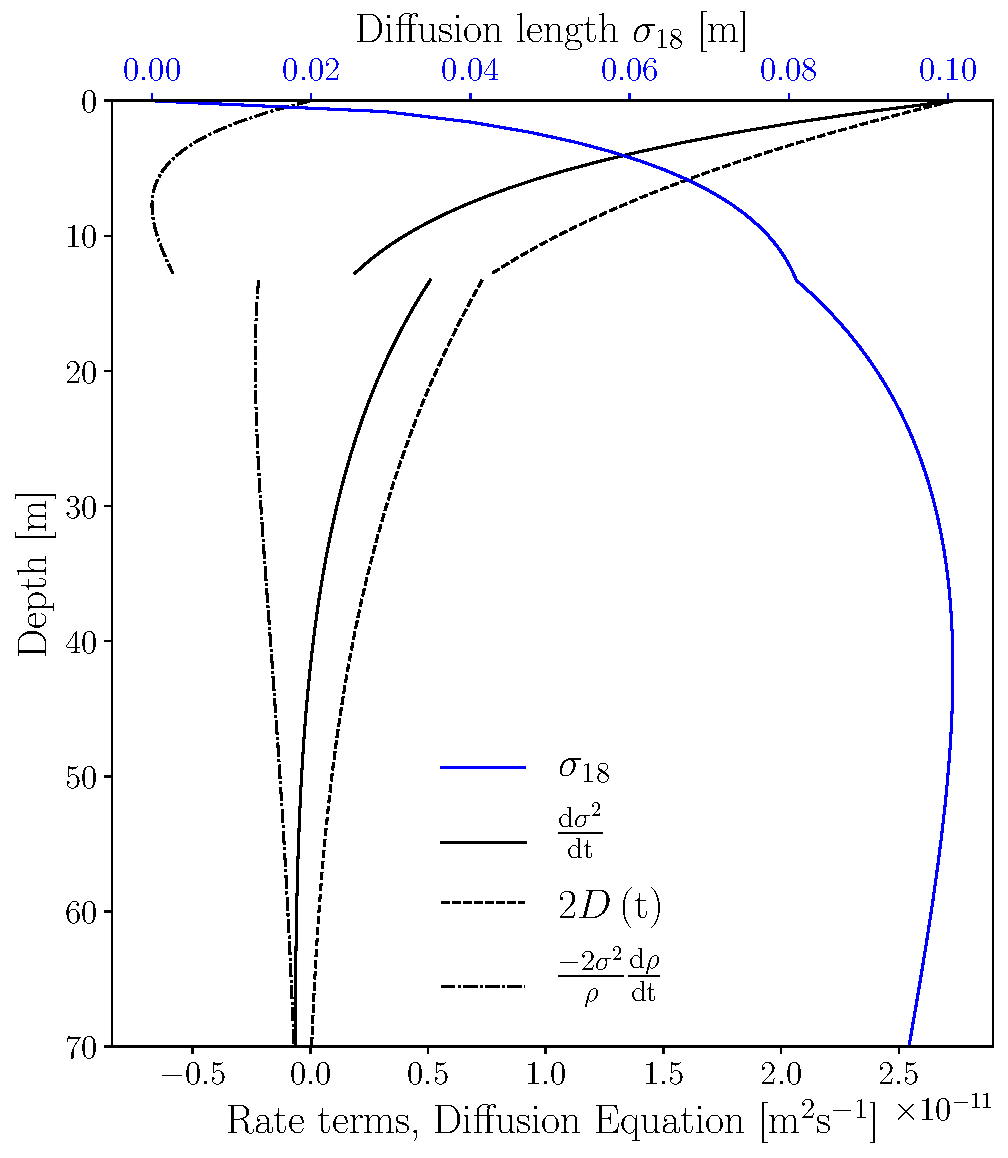
\includegraphics[width=0.6\textwidth]{Analytical_DiffLenEq_terms_SiteA.pdf}
	\caption[Rate terms in the diffusion equation.]{\small Contribution of the diffusion(dashed) and densification(dot-dashed) terms from Eq. \ref{Eq:dsigma2_dt} to the final analytical diffusion length solution (blue).}
	\label{Fig:ICE_DiffDensTerms}
\end{figure}

To simplify the work of this thesis, the numerical module of the CFM and the iso-CFM has not been implemented in the final computations, and the diffusion length profiles referred to in the rest of the project are calculated through an analytical method, using equations derived from Eq. \ref{Eq:dsigma2_dt} analytically. A short walk-through of the derivations are presented in Appendix \ref{AppIX:CFM} as they are described in \cite[Gkinis et al., 2021]{Gkinis2021}. Five examples of diffusion length profiles given different conditions are presented in Figure \ref{Fig:DiffProf_Examples}, with the same conditions as used in \ref{Fig:DensProf_Examples}.

The analytical equations derived in Appendix \ref{AppIX:CFM} have been used for creating a contour plot of the analytical solutions for $\sigma_{18}$ at the close-off density, $\rho_{\text{co}}$. This can be seen in Figure \ref{Fig:ICE_ContourPlot}. The plot shows six different ice cores drilled in the proximity of the Crête ice core drill site and their diffusion length analytical solutions.

\begin{figure}
	\centering
	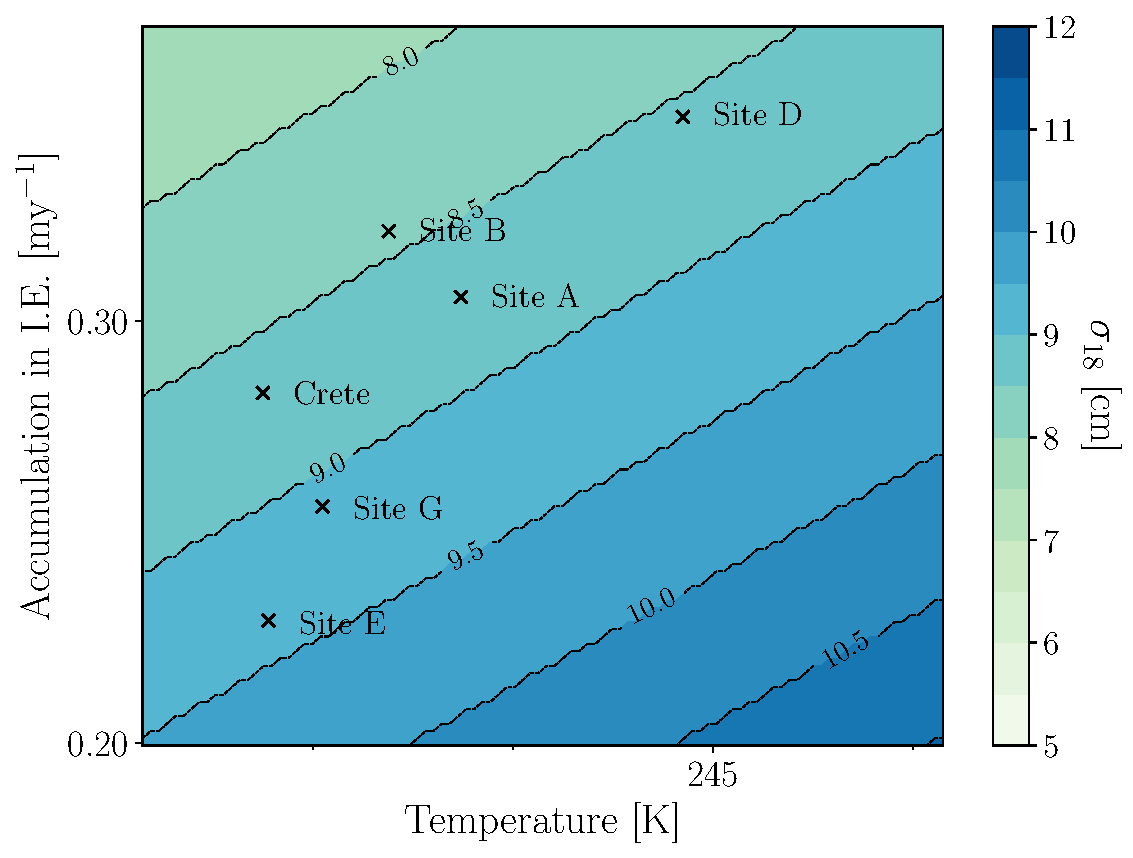
\includegraphics[width=0.7\textwidth]{ContourPlot_Alphabet.pdf}
	\caption[Analytical solutions of diffusion length, Alphabet cores.]{\small Crete and surrounding Alphabet cores, as their analytical solutions place them according to observed temperature and accumulation rate.}
	\label{Fig:ICE_ContourPlot}
\end{figure}


These analytical equations are used to compute diffusion lengths to compare with the optimal diffusion length estimates computed from the raw data. One could advantageously explore the iso-CFM further to numerically compute the diffusion lengths with different temperature and accumulation forcing to recreate a diffusion length profile corresponding to the most likely at a given drill site. Since the iso-CFM do consist of many different modules all with different possibilities for parameterisation, it is outside the scope of this project to develop more advanced iso-CFM diffusion length estimates for the examined cores, and only the previously described, simple diffusion length profile estimate will be used in the further work. In-depth methodology and results from the iso-CFM can be found in \cite[Gkinis et al., 2021]{Gkinis2021}.

\begin{marginfigure}
	\centering
	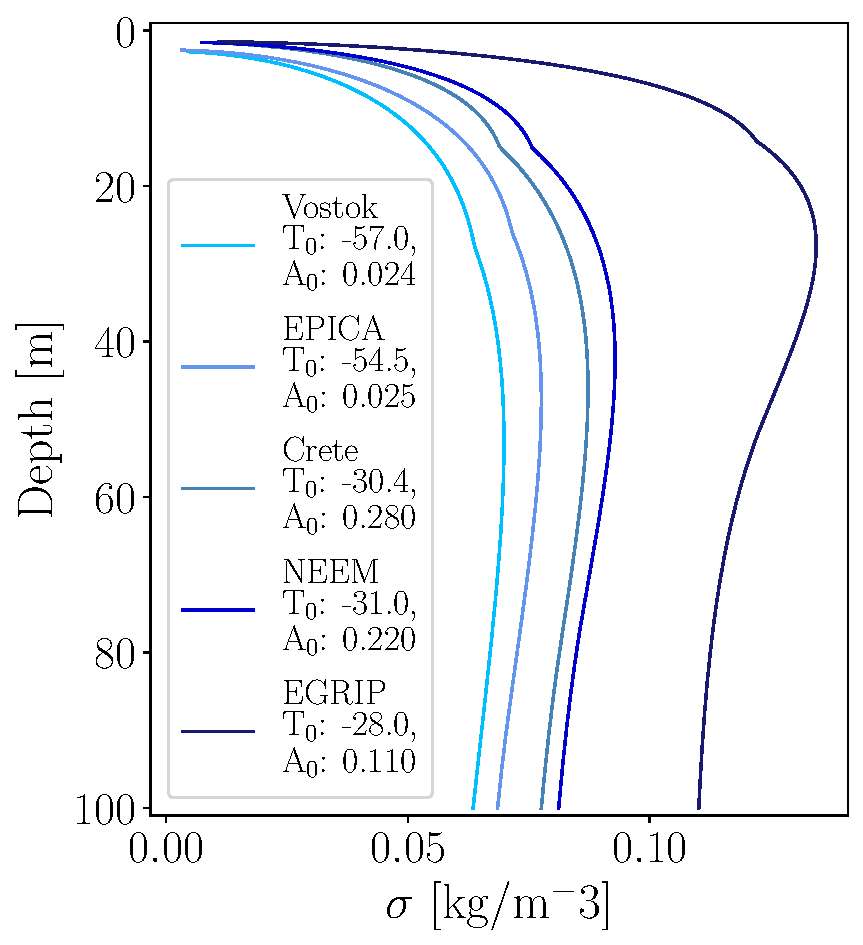
\includegraphics[width=\marginparwidth]{DiffProf_Examples.pdf}
	\caption[Five different analytical diffusion length profiles.]{\footnotesize Analytically calculated diffusion length profile examples given five different initial conditions representing present day conditions at the five different ice core locations. Temperature, $T_0$, is in $^{\text{o}}$C and accumulation, $A_0$, is in meter of water equivalent per year.}
	\label{Fig:DiffProf_Examples}
\end{marginfigure}

\section[Temperature Estimation]{Temperature Estimation}
\label{Sec:Ice_TempEstimation}

Through the theoretically based analytical (or nummerical) estimates of the diffusion length, $\sigma_{\text{model}}$, and the diffusion length estimate from the isotopic signal of a depth section of an ice core, $\sigma_{\text{firn}}$, a temperature estimate of can be given. This estimate made by numerically solving Eq. \ref{Eq:Firn_Temp_est_Roots} with $T$ as the unknown variable:
\begin{equation}
	\left(\frac{\rho_{\text{co}}}{\rho_{\text{ice}}}\right)^2 \sigma_{\text{model}}^2(\rho=\rho_{\text{co}}, T(z), A(z)) = \sigma^2_{\text{firn}}.
	\label{Eq:Firn_Temp_est_Roots2}
\end{equation}

For the temperature estimates made in this project a secant numerical method\cite{Press2007} was used, through the Python \lstinline[language=Python]|SciPy| package \lstinline[language=Python]|scipy.optimize.newton|. Only the function it self is provided and no derivative is given, so the \lstinline[language=Python]|scipy.optimize.newton| uses the secant method to find a zero of the function passed. If a derivative was given, the packages would use a Newton-Raphson\cite{Press2007} scheme to find the zero of the function.


%\todo{ICE-TEMP.EST: Give an example of temperature estimation?}





\section[ECM and DEP][ECM and DEP]{Dating of Ice Cores: ECM and DEP}
\label{Sec:Ice_ECMandDEP}

\begin{figure}[h]
	\centering
	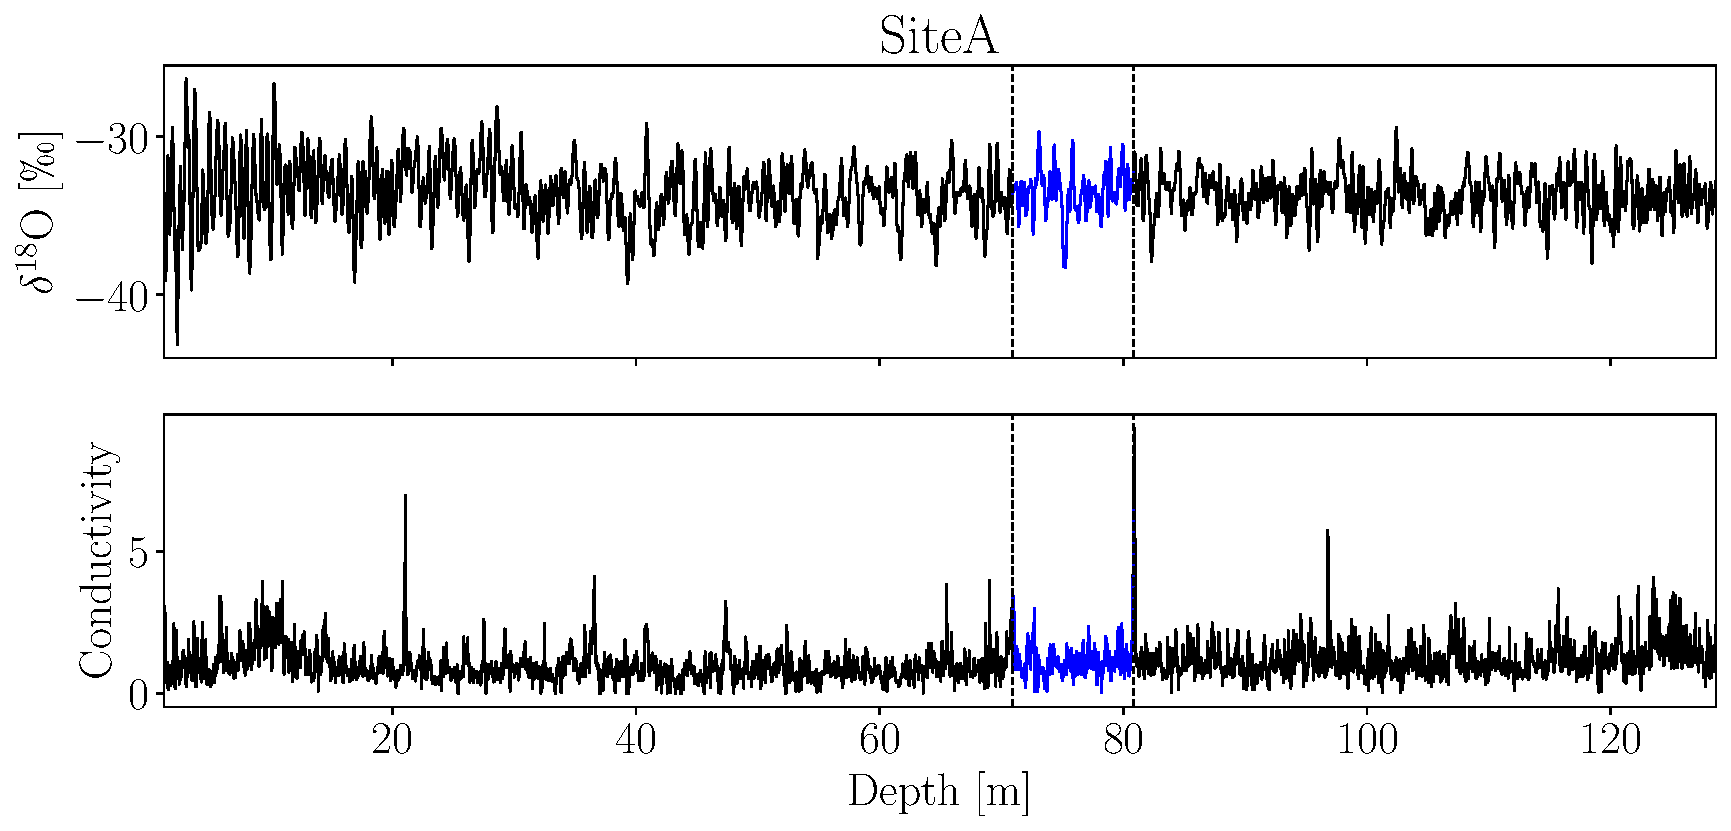
\includegraphics[width=\textwidth]{SiteA_ECM_d18O_full.pdf}
	\caption[Conductivity and $\delta^{18}$O measurements from Site A.]{\small Water isotope measurements aligned with conductivity measurements from the ice core drilled at Site A.}
	\label{Fig:ICE_SiteA_ECM_d18O_full}
\end{figure}

Isotopic composition analysis has already been presented as a tool for analyzing ice cores to examine past temperatures, climate and atmospheric composition. Another method is through electrical conductivity measurements(ECM) which is much more sensitive to violent volcanic eruptions and deposition of volcanic material. This sensitivity makes it possible to use historically dated eruptions visible in the ice cores as volcanic horizons, and thus making dating of the ice core more precise and absolute. In Figure \ref{Fig:ICE_SiteA_ECM_d18O_full} two aligned depth series can be seen: the water isotope profile and the conductivity profile. The conductivity profile shows clear peaks, which are a result of the increased conductivity due to volcanic material deposited along with the snow at the ice core drill site.


\subsection[ECM][ECM]{Electrical Conductivity Measurements}
\label{Sec:Ice_ECMandDEP_ECM}


The conductivity of ice arises from the current emerging due to the build-up of space charges in the ice structure. This conductivity can be analyzed by measuring the electrical current(DC) - induced by the electric potential and the acid balance - between two electrodes which are moved along the ice cores length. This current will be connected to the acid impurity concentration (pH), in the form of $\text{H}_3\text{O}^+$ concentration, of the ice core. Higher levels of acid impurity concentration are due to volcanic eruptions. Large amounts of volcanic gases, i.e. $\text{SO}_2$, in the atmosphere oxidizes and combines with water to form acid, i.e. sulphuric acid, which is then washed out of the air due to precipitation. Thus it is made possible to recognize volcanic horizons in ice cores, and - if the spatial location of the eruption is known - from the amount of acid, the magnitude of the eruption can also be estimated.

%High acidity of layers containing volcanic fall-out influences the dielectric constant of ice, so that these layers may be a possible explanation to the internal reflection horizons found in radio-echo sounding. 

The measured current can then be transformed into acidity by a calibration curve relating the current, in $\mu$A, to the acidity, in $\mu$equivalents $\text{H}_3\text{O}^+$ per kilogram. To find the calibration parameters, the current and the acidity must be measured - the current through the above mentioned method, and the acidity through pH measurements of melted ice core samples. The pH measurements must further be corrected for any $\text{co}_2$ induced $\text{H}^+$ ions (REFERENCES).The relation between acidity [$\text{H}^+$] (corrected for $\text{co}_2$ induced $\text{H}^+$) and current $I$ can be expressed in two ways:
\begin{itemize}
	\item $[H^+] = (0.017\, I^2 + 1.2) \mu \text{equiv. H}^+ /\text{kg}$\\
	without a 50\% correction for $\text{co}_2$ surplus.
	\item $[H^+] = (0.045\, I^{1.73}) \mu \text{equiv. H}^+ /\text{kg}$\\
	with a 50\% correction for $\text{co}_2$ surplus.
\end{itemize}
The salt concentration in the ice can be estimated from measurements of the specific conductivity $\sigma$ of the melted samples. The salt contribution hereto can be expressed as:
\begin{equation}
	\sigma_s = \sigma - \sigma(\text{H}^+) - \sigma(X^-) - \sigma(\text{HCO}_3^-)
\end{equation}
where the three later terms correspond to the contributions from $\text{H}^+$(through pH measurements) and its anions\footnotemark, $\text{HCO}_3^-$ and any other anions $X^-$. The anion concentration will be equal to the cation concentration, which in this case is only $\text{H}^+$ concentration. Disregarding low acidity samples, the concentration of $\text{HCO}_3^-$ is negligible and thus  $\text{concentration}(X^-) \approx \text{concentration}(\text{H}^+)$. 
The current is thus heavily influenced on/determined by the $\text{H}^+$ concentration, and thus it is approximated that the salt concentration has no influence on the current readings, which is fortunate, since the ECM method only responds to acidity, and not to salt and ammonia concentrations. This is one of the method's limitations, which the later dielectric profiling (see Appendix \ref{AppX:DEP}) method has taken into account.

\footnotetext[2]{Anions are molecules losing a number of electrons to become negatively charged. Cations are molecules that gain a number of electrons to become positively charged.}

Though DEP measurements might have been more sensitive to salt and ammonia concentrations and thus would have given a different signal, the data available for conductivity for the ice cores under consideration in this thesis are made through the ECM method. In Figure \ref{Fig:ICE_SiteA_ECM} the raw ECM signal can be seen, aligned with the isotopic signal. Marked in blue is the estimated depth between the two eruptions Laki and Tambora.



%\subsection[Volcanic Horizons][Volcanic Horizons]{Dating of Ice Cores Through Volcanic Horizons}
%\label{Subsec:Ice_ECMandDEP_VolcanicHorizons}


%\begin{figure}[h]
%	\centering
%	\begin{subfigure}{.8\textwidth}
%		\centering
%		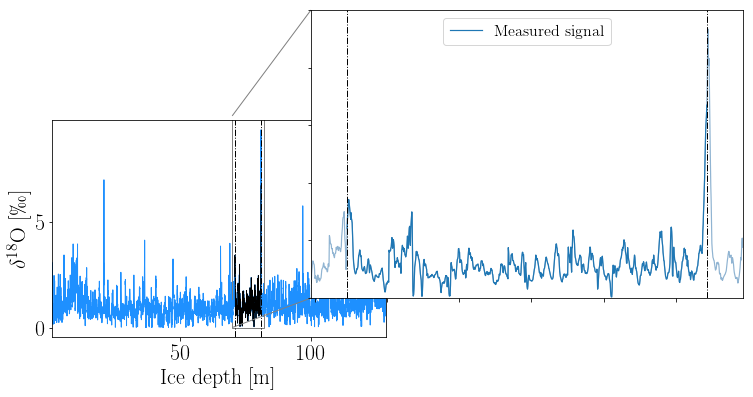
\includegraphics[width=\textwidth]{SiteA_ECMInsert.png}
%		\caption{Electrical Conductivity Measurements (ECM) from Site A with a zoom-in on the depth section corresponding to the time between the volcanic eruptions of Tambora and Laki}
%		\label{fig:SiteA_ECMInsert}
%	\end{subfigure}
%	~
%	\begin{subfigure}{.8\textwidth}
%		\centering
%		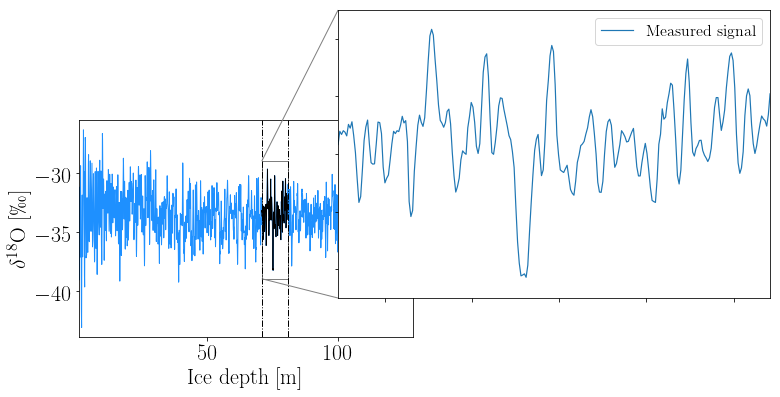
\includegraphics[width=\textwidth]{SiteA_d18OInsert.png}
%		\caption{Water isotopic signal from Site A with a zoom-in on the depth section corresponding to the time between the volcanic eruptions of Tambora and Laki}
%		\label{fig:SiteA_d18OInsert}
%	\end{subfigure}
%	\caption{Isotopic and ECM signals, with a focus on the depth sections between eruptions from Tambora and Laki.}
%	\label{fig:SiteA_d18O_ECM}
%\end{figure}
%Throughout the history of the earth a number of different geophysicals events have left their mark on the geological and glaciological records we use to steal a glance into the past. When considering ice core records, there are few as visible - both to the eye and in measured data - than volcanic eruptions. It is widely known [REFERENCE] that eruptions above a certain scale have the possibility to change not only the atmospheric composition, due to the heavy amount of volcanic material slung into the air, but also the ability to impact the climate in the years following an enormous eruption. 

Through electrical conductivity measurements it is possible to observe the very clear effects of some volcanic events in ice cores. Particles from the eruption are quickly transported from the source, since the atmospheric airflow will scatter the particles all over the atmosphere at a relatively high speed. Thus the dust(particle) and ECM signals pick up the volcanic signal faster than for example the isotopic signals. The isotopic signal reacts much slower, as it must be subjected to a change in global - and then following local - temperature, which might first show after a number of years. Thus ECM, DEP and dust measurements are good records to use for dating ice cores. Some eruptions are only great enough to show in ice cores located close to the volcanic source [REFERENCE], while others are of a magnitude impacting the entire globe, thus showing in almost all ice core records. These volcanic horizons are specifically good for synchronizing records, which is essential for developing knowledge about the geographically varying climate, temperatures and hemispherical dependency of the past. 






\end{document}